% Ear as a Hydrophone. IEEE ICCE 2027 (Las Vegas), IEEE conference template.
% Draft for co-authors. Red [TODO] marks are open.
\documentclass[conference]{IEEEtran}
\IEEEoverridecommandlockouts
\usepackage{cite}
\usepackage{amsmath,amssymb}
\usepackage{graphicx}
\usepackage{booktabs}
\usepackage{xcolor}
\usepackage{url}
\usepackage[hidelinks]{hyperref}
\graphicspath{{figures/}}

\newcommand{\todo}[1]{\textcolor{red}{[TODO: #1]}}

\begin{document}

\title{Ear as a Hydrophone: Listening to a Hydraulophone Through the Water with a Consumer EEG and fNIRS Headband}

\author{
\IEEEauthorblockN{Alexander Vicol and Steve Mann}
\IEEEauthorblockA{University of Toronto and MannLab Canada, Toronto, Canada\\
vicola.lexo@gmail.com}
}

\maketitle

\begin{abstract}
The eye as a camera reads a picture from the visual cortex while the eye looks at a flickering target. The ear as a hydrophone is the same idea turned to the water: the listener puts an ear to the surface, the sound of an instrument played in the water reaches it through the water rather than the air, and a headband on the listener records what the head does with it. We report the first such recording. The second author lay at the edge of a dock with his ear at the water while a hydraulophone, the water-jet instrument he invented, was played beside him, wearing a Muse S Athena headband that logs four EEG channels and sixteen optical channels. Six minutes, no markers. The EEG was usable on 92 to 100\% of two-second epochs, at 13 to 27\,$\mu$V rms, with no narrow spectral line that moved with the music and one steady 64\,Hz line that is the headband's own optical clock. The optical channels carried a clean pulse at 64 beats per minute, the same on both temples, a breathing rhythm near 7 per minute, and a rise in oxygenated haemoglobin through the six minutes on every detector pair with deoxygenated haemoglobin flat, the signature of a head held below the heart rather than of listening. A hydraulophone's notes lie above the headband's 128\,Hz Nyquist limit, so what the EEG can carry of the sound is not the note but the auditory steady-state response to its modulation; from the measured floor at 40\,Hz we compute that a 0.3\,$\mu$V response would need three clean minutes to reach a signal-to-noise ratio of three, and we set out the tagged-note protocol that would deliver it. The paper is a feasibility account and a protocol, not a result about hearing.
\end{abstract}

\begin{IEEEkeywords}
hydraulophone; underwater hearing; auditory steady-state response; EEG; fNIRS; photoplethysmography; wearable computing; consumer electronics; Mersivity.
\end{IEEEkeywords}

\section{Introduction}

The hydraulophone is a musical instrument whose keys are water jets: the player's fingers block or divert the jets, and the sound is made in the water and carried by it \cite{mann2005fluid, mann2006hydraulophone, mann2007physiphones}. It is the one instrument whose sound a listener can hear best with the ear in the water, which is where its player's hands already are. Human hearing under water is bone conduction, with thresholds some 30 to 60\,dB above those in air and a frequency response that favours the low kilohertz \cite{brandt1967underwater, hollien1969underwater}; the ear is a poor hydrophone, but it is one.

Our eye-as-camera work \cite{mann2019eye} and its consumer-hardware sequel read what the visual cortex does with a flickering target from a headband and one added electrode. The ear-as-hydrophone question is its auditory twin: what does a consumer headband record from a head that is listening through the water? Two signals are available. The EEG carries the auditory steady-state response (ASSR), the cortical following of a sound's amplitude modulation, strongest near 40\,Hz \cite{galambos1981assr, picton2003assr}; and the headband's optical channels carry the pulse, the breathing, and the slow haemodynamics of the forehead \cite{allen2007ppg, scholkmann2014fnirs}, which a listening or a breath-holding head changes. The Muse S Athena logs both from the same band \cite{krigolson2017muse}.

This paper reports the first recording of the kind, taken outdoors at a dock on October 4, 2026 (Fig.~\ref{fig:photo}), and asks the same question our Vehicraft paper asks of the water: what did the headband actually give, and what would the next recording need. There are no markers and no stimulus log, so there is no response to report; there is the measurement, and the protocol it leads to.

\begin{figure}[t]
\centering
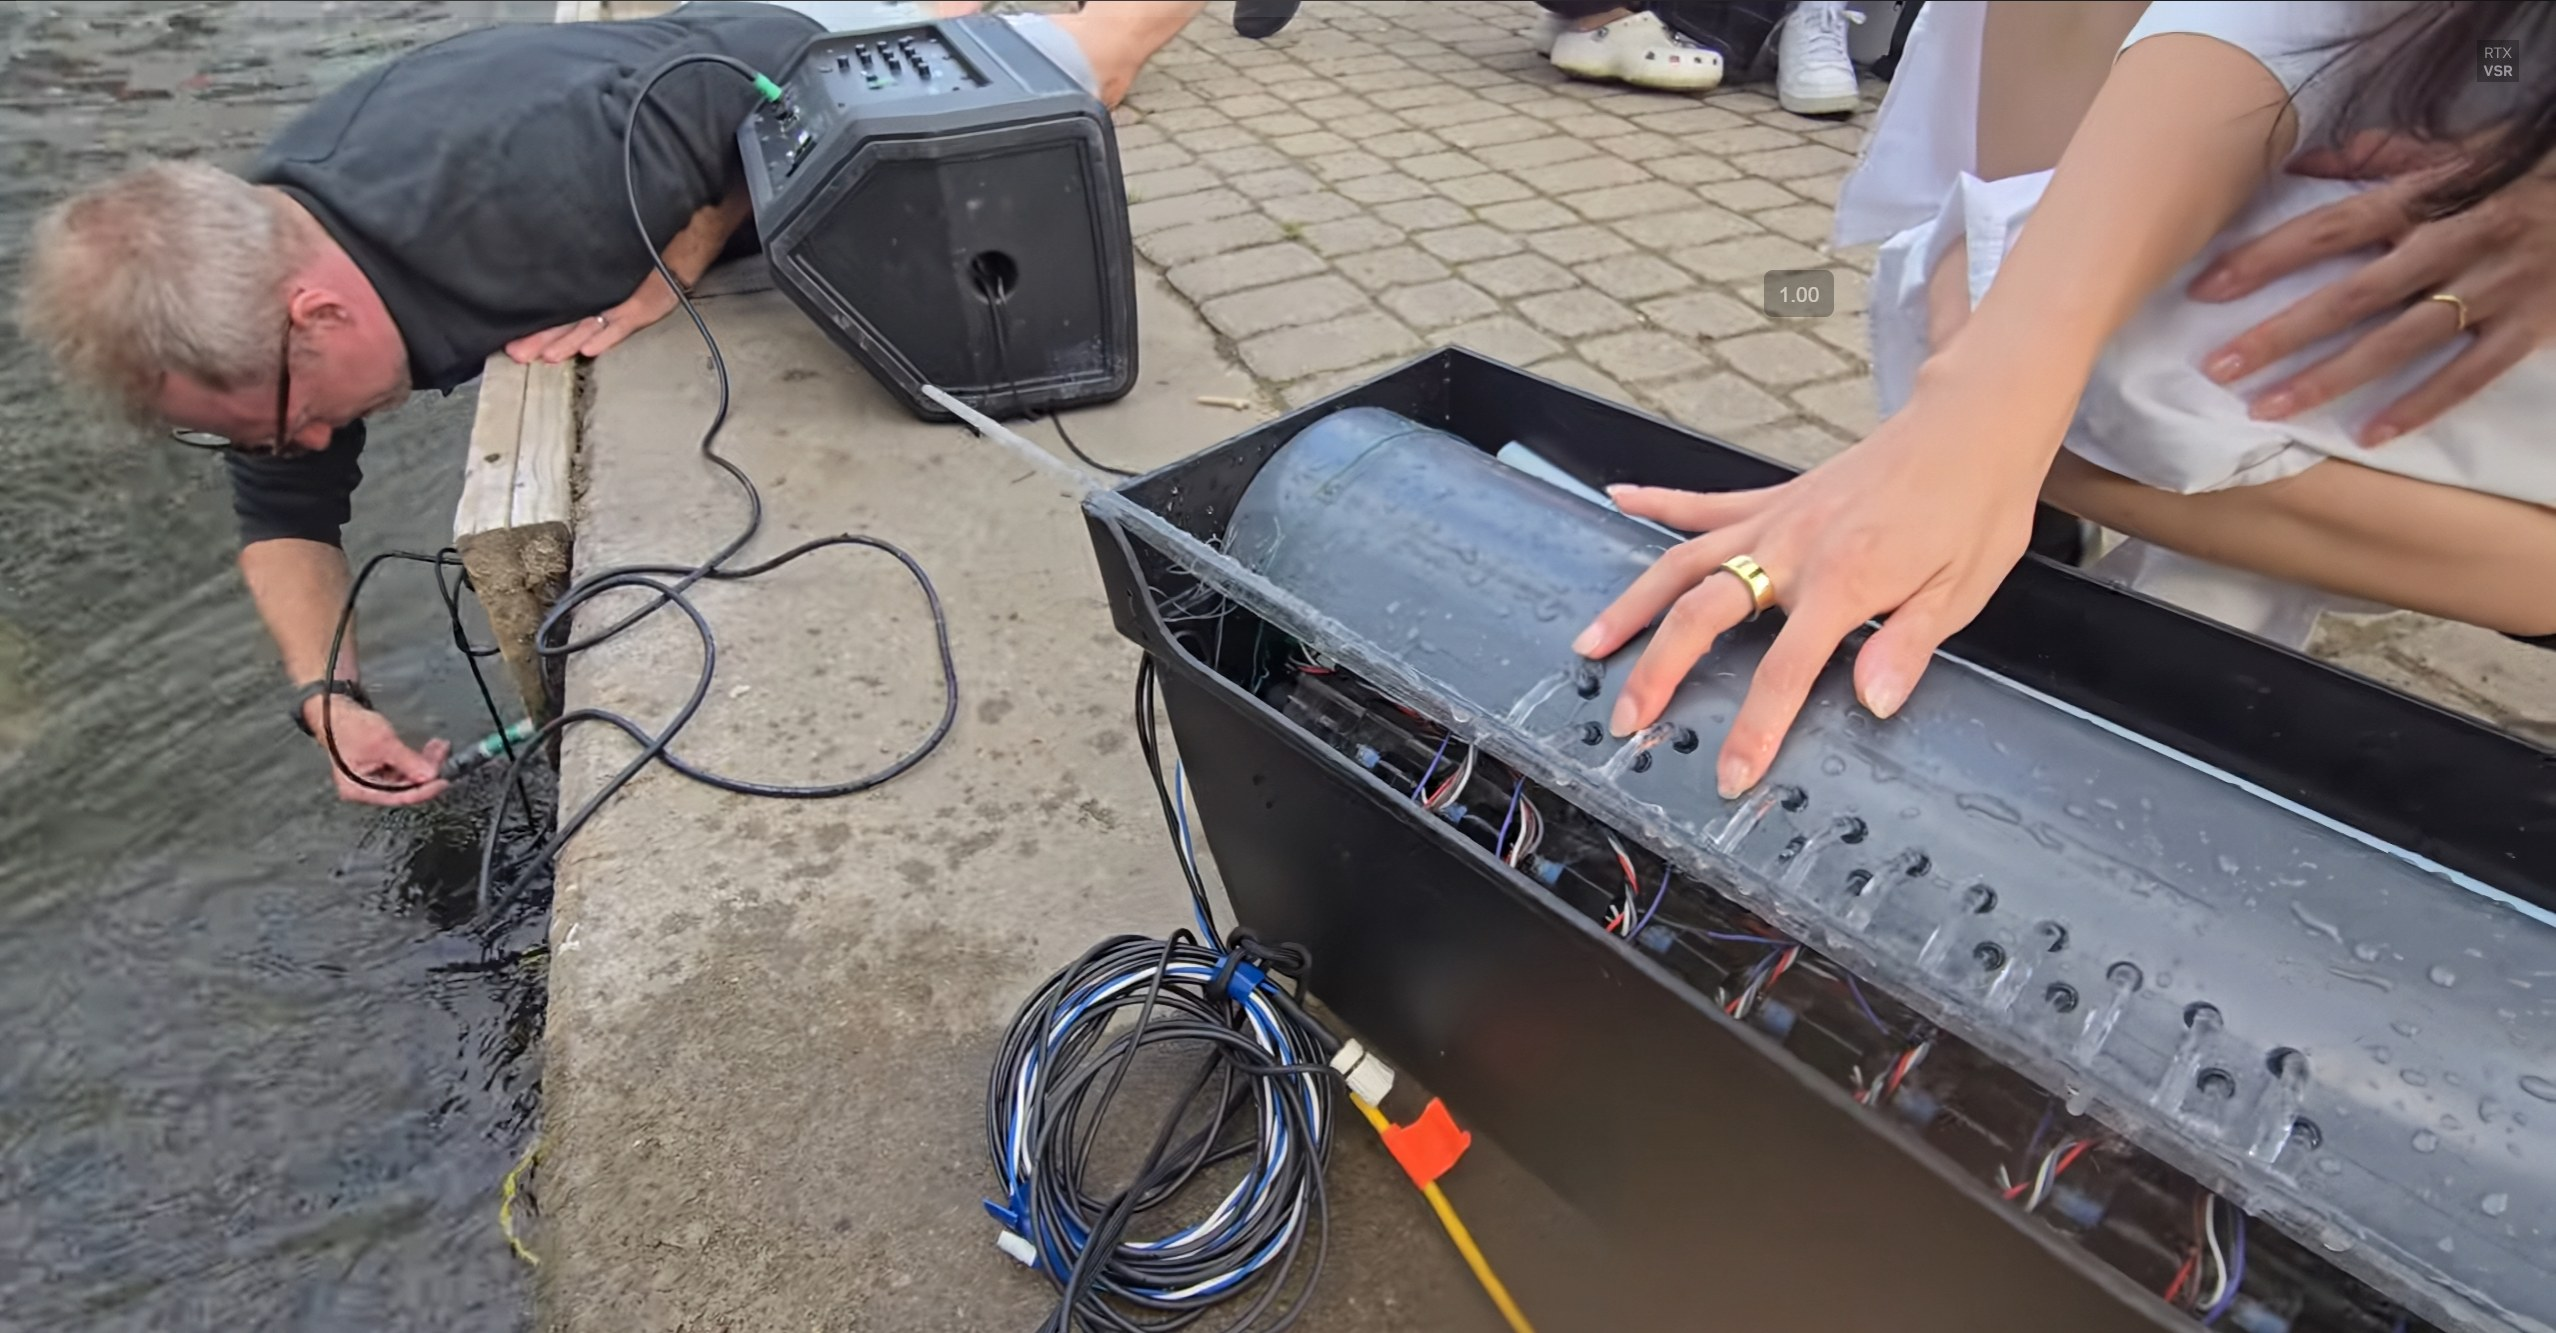
\includegraphics[width=\columnwidth]{photo_dock}
\caption{The recording: the second author lies at the edge of the dock with his ear at the water, holding the lead that runs into it, wearing the headband. The hydraulophone, its jets in the trough with their pickups wired below, is played beside him; the amplifier sits on the dock behind.}
\label{fig:photo}
\end{figure}

\section{Methods}

\textbf{Recording.} Muse S Athena headband: four dry EEG electrodes at TP9, AF7, AF8 and TP10 referenced at Fpz, sampled at 256\,Hz, and an optical array of two detector distances (inner and outer) on each temple at 730 and 850\,nm with red and ambient references, streamed over Bluetooth to a phone running MuseLog, which writes one row per EEG sample with the optical samples held between their own updates. 6.3 minutes, 16:37 to 16:44. No trigger was pressed; the hydraulophone was played throughout with pauses. \todo{who played, what was played, how far the ear was in the water, whether the lead in the water is a hydrophone feeding the amplifier}

\textbf{EEG.} Channels band-passed 1 to 125\,Hz and cut into 2\,s epochs, usable under 200\,$\mu$V peak. Spectra are Welch estimates over the usable epochs with 8\,s segments. A steady line is a bin that is a local maximum and at least five times the median of its 0.6 to 3.5\,Hz neighbourhood; its amplitude is the power above that floor expressed as a sinusoid's rms. A spectrogram (4\,s windows, 1\,s step) is searched for ridges, narrow peaks that move in frequency from one window to the next, which is what a played note would leave if any of its energy fell below 128\,Hz. Alpha and the broadband level on the ear channels are followed per 10\,s.

\textbf{Optical.} The optical series are low-passed and decimated to 32\,Hz. The pulse is read on the 850\,nm inner channel of each temple, band-passed 0.7 to 3\,Hz: the Welch peak over the whole file as heart rate, and the peak per 20\,s window as its course. Breathing is the 0.1 to 0.5\,Hz peak on the same channel. Oxygenated and deoxygenated haemoglobin changes come from the 730 and 850\,nm pair of each detector by the modified Beer-Lambert law with approximate extinction coefficients, in relative units, smoothed over 10\,s \cite{scholkmann2014fnirs}.

\textbf{Budget.} For an ASSR of rms amplitude $A$ over a measured floor $N$ (in $\mu$V$^2$/Hz) the clean recording time to reach a signal-to-noise ratio $s$ in one spectral bin is $T = sN/A^2$ seconds, since the signal's bin power is $A^2$ and the noise's is $N/T$.

\section{Results}

\textbf{The EEG held.} Table~\ref{tab:eeg}. Lying still with the head at the water, the headband gave usable EEG on 92\% of epochs behind the left ear, 96\% behind the right, and 99 to 100\% on the forehead, at 26 to 27\,$\mu$V rms behind the ears and 13 to 16 on the forehead. That is a better recording than any of the three the same headband gave on the same harbour five days later from a moving craft, and as good as our indoor sessions. Mains pick-up at 60\,Hz was 0.4 to 3\,$\mu$V$^2$/Hz, low, as outdoors it should be.

\begin{table}[t]
\caption{What the EEG gave. Usable epochs are 2\,s epochs under 200\,$\mu$V; rms is over the usable epochs, 1 to 125\,Hz; alpha is 8 to 13\,Hz; the floor is the median power at 37 to 43\,Hz, where an ASSR would sit.}
\label{tab:eeg}
\centering
\scriptsize
\setlength{\tabcolsep}{5pt}
\begin{tabular}{lcccc}
\toprule
channel & usable & rms, $\mu$V & alpha, $\mu$V$^2$/Hz & floor at 40\,Hz \\
\midrule
TP9, left ear & 92\% & 27 & 6.2 & 4.9 \\
AF7, left forehead & 99\% & 16 & 1.3 & 3.1 \\
AF8, right forehead & 100\% & 13 & 0.9 & 0.7 \\
TP10, right ear & 96\% & 26 & 6.9 & 4.1 \\
\bottomrule
\end{tabular}
\end{table}

\textbf{No note in the EEG, and one line that is the headband's.} Fig.~\ref{fig:spectra} and~\ref{fig:specgram}. The whole-file spectra are the ordinary 1/f shape with a small alpha shoulder behind the ears. The spectrogram shows no ridge that moves with the music: the structure in it is vertical, the broadband bursts of a head and a jaw that move, not horizontal lines that step from note to note. That is what the headband's sampling predicts. A hydraulophone's fundamentals run from the low hundreds of hertz upward, every one of them above the 128\,Hz Nyquist limit of a 256\,Hz headband, and what folds back from them is spread, not a line. The one steady line in the recording is at 63.9\,Hz, present in every window on every channel, strongest on the right forehead at about 1\,$\mu$V rms. It is not the mains, which sits at 60\,Hz and is weaker; it is at the optical sampling rate of the Athena, it is absent from the three recordings we made with the optical stream not logged, and it should be read as the headband's own LEDs seen by its own electrodes.

\begin{figure}[t]
\centering
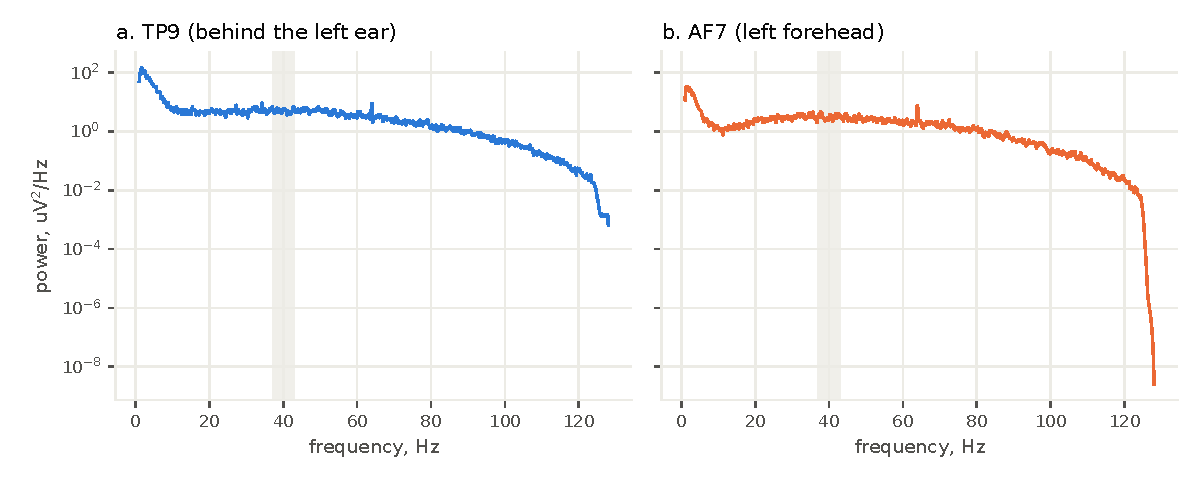
\includegraphics[width=\columnwidth]{fig_spectra}
\caption{Spectra of the usable epochs behind the left ear and on the left forehead. The band at 37 to 43\,Hz is where an auditory steady-state response to a 40\,Hz modulation would appear; the labelled line at 64\,Hz is the headband's optical clock.}
\label{fig:spectra}
\end{figure}

\begin{figure}[t]
\centering
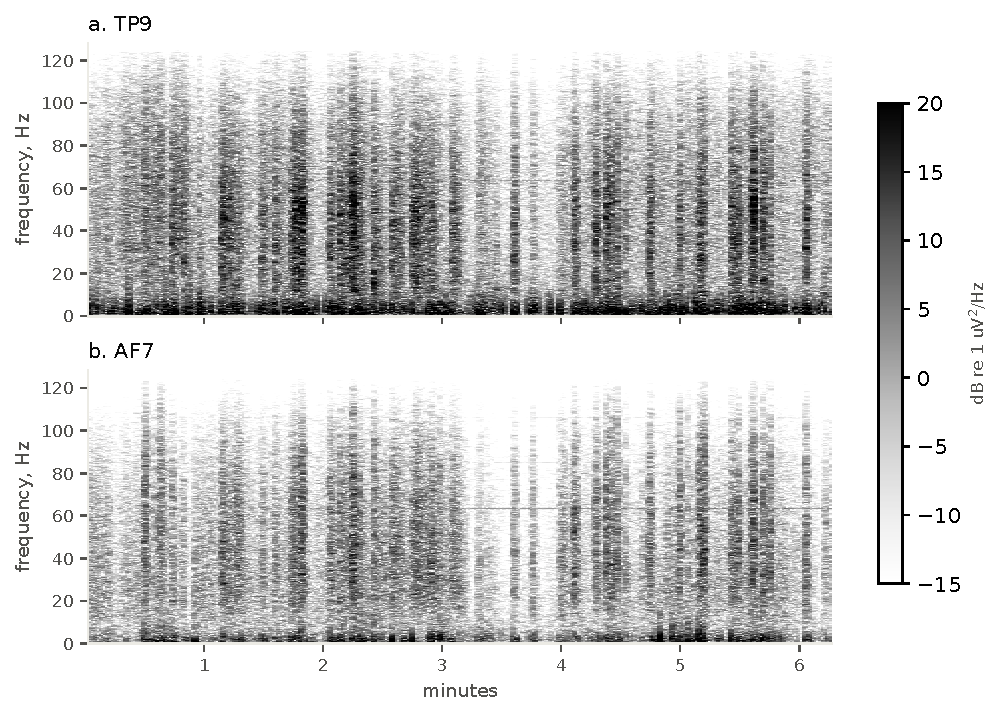
\includegraphics[width=\columnwidth]{fig_spectrogram}
\caption{Spectrograms of the same two channels through the six minutes. The structure is vertical (movement) and the one horizontal line is at 64\,Hz; nothing steps from note to note.}
\label{fig:specgram}
\end{figure}

\textbf{Alpha and the level through the session.} Fig.~\ref{fig:course}. Alpha behind the ears swung between 3 and 14\,$\mu$V$^2$/Hz from one 10\,s window to the next and drifted from about 7 in the first minute to 4 in the last; the broadband level stayed at 25 to 26\,$\mu$V. There is no eyes-closed plateau and no sign of a settled, listening state in the EEG alone, which is what six minutes of an unmarked outdoor recording of a head that is talking and moving should look like.

\begin{figure}[t]
\centering
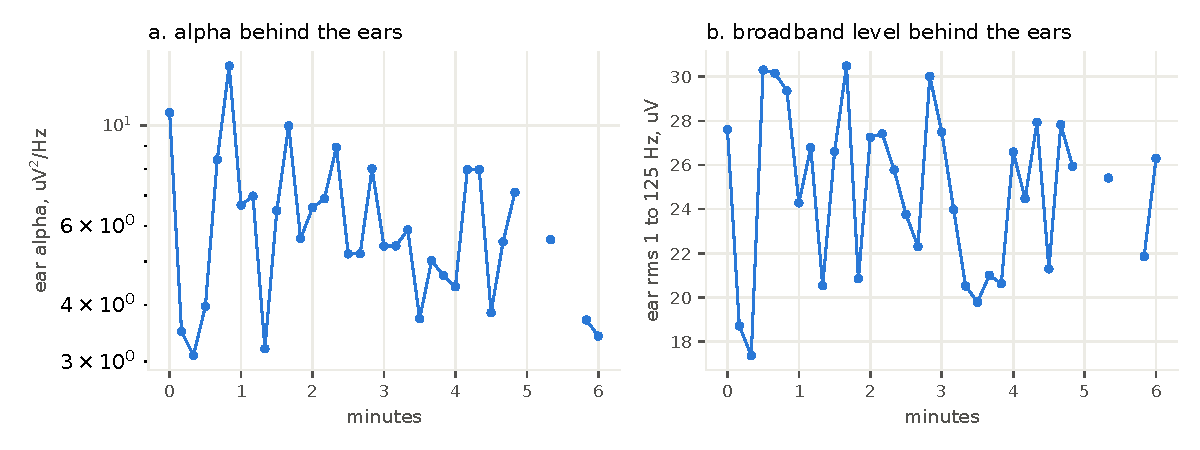
\includegraphics[width=\columnwidth]{fig_timecourse}
\caption{Alpha (left) and the broadband level (right) behind the ears per 10\,s through the recording; gaps are windows with an artifact on both ear channels.}
\label{fig:course}
\end{figure}

\textbf{The optical channels carried the body.} Fig.~\ref{fig:optics}. The 850\,nm inner channel on each temple shows a pulse at 1.07\,Hz, 64 beats per minute, a hundred times its neighbouring spectrum, at 1.2\% of the mean light on the left and 0.95\% on the right, with the beat-to-beat waveform visible by eye. The rate per 20\,s held at 60 to 66 through the session with one window at 78. The slow band shows a breathing rhythm at 0.12\,Hz, about seven breaths a minute, slower than resting breathing, which is what a listener with the face at the water does. Oxygenated haemoglobin rose through the six minutes on all four detector pairs, by 0.08 to 0.11 relative units from the first minute to the last, with deoxygenated haemoglobin flat or slightly falling, the same on the left and the right and at the short and the long detector distance. A change that is equal on every pair and at every distance is not a cortical response; it is the forehead's blood volume rising as the head is held below the heart, the posture of Fig.~\ref{fig:photo}.

\begin{figure}[t]
\centering
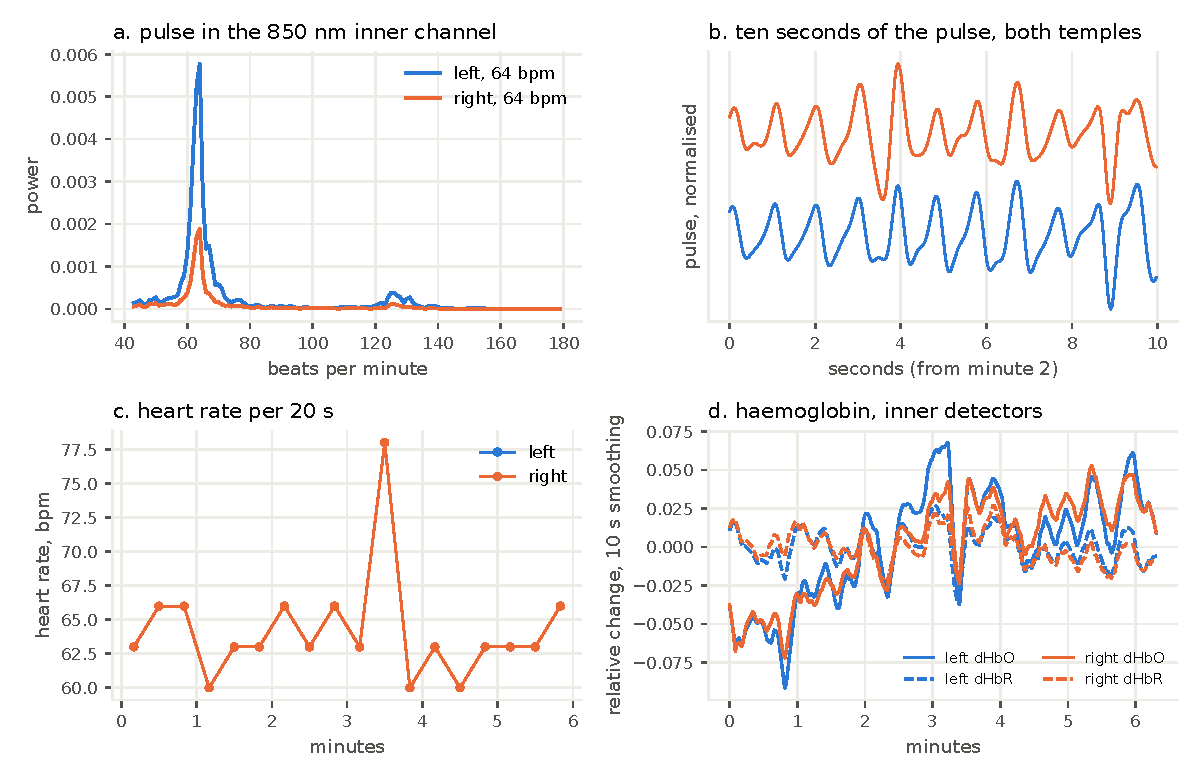
\includegraphics[width=\columnwidth]{fig_optics}
\caption{The optical channels. a: the pulse spectrum of the 850\,nm inner channel on each temple, peaking at 64 beats per minute. b: ten seconds of the pulse waveform from minute two. c: heart rate per 20\,s. d: oxygenated (solid) and deoxygenated (dashed) haemoglobin change on the inner detectors, relative units, through the recording.}
\label{fig:optics}
\end{figure}

\textbf{What a response would need.} Fig.~\ref{fig:budget}. The floor behind the ears at 37 to 43\,Hz was 4.1 to 4.9\,$\mu$V$^2$/Hz, 4.5 on average. A 40\,Hz ASSR of 0.5\,$\mu$V rms, the upper end of what scalp recordings give to a loud modulated tone \cite{picton2003assr}, would reach a signal-to-noise ratio of three in a single bin in about one clean minute; 0.3\,$\mu$V in three minutes; 0.2\,$\mu$V in six. Our own attempt at a 40\,Hz response indoors, with a cup electrode at the vertex and earbuds, found nothing in nineteen tagged and nineteen plain blocks and put any response below about 0.3\,$\mu$V. Under water the sound reaches the cochlea by bone at a lower level, so the response, if it is there, will be at the small end of that range, and the clean minutes must be minutes with the head still.

\begin{figure}[t]
\centering
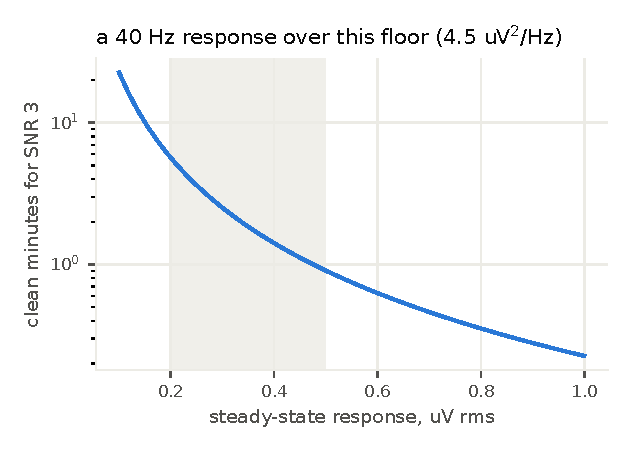
\includegraphics[width=0.8\columnwidth]{fig_budget}
\caption{Clean recording time for a 40\,Hz steady-state response to reach a signal-to-noise ratio of three over the floor measured behind the ears, against the response's amplitude. The band marks the range scalp recordings report.}
\label{fig:budget}
\end{figure}

\section{The Protocol This Leads To}

The recording tells us what to change, and the stimulus page we built for the eye already does most of it. \emph{A tagged note.} Play one hydraulophone jet, or the amplifier driving a transducer in the water, with its amplitude modulated at a rate the headband can see, 40\,Hz first, in blocks of 8\,s on and 8\,s off, twenty of each, with the block edges logged; the ASSR is then a line at 40\,Hz that is present in the on blocks and absent in the off blocks, and an exact permutation test over the block labels decides it, exactly as our visual calibration does for flicker. \emph{A trigger per condition.} Ear in the water, ear out of the water, ear plugged in the water, each for the same blocks, so that the water path is the contrast and not the music. \emph{A still head.} The head on a rest at the water, because the budget is in clean minutes and a moving head spends them. \emph{The optical stream as the second channel.} The pulse and the breathing come free and are the listener's state; a breath-hold under water shows in both and must be logged rather than discovered. \emph{A cup electrode.} At the vertex for the ASSR, as our indoor attempt used, since the Muse's ear sites are also where the water is. Three such sessions, each under half an hour, turn the question into a number with an interval around it.

\textbf{Limits.} One listener, one afternoon, six minutes, no markers, no stimulus log, no baseline out of the water. Nothing here is a measurement of underwater hearing. The 64\,Hz line's attribution to the optical clock rests on its absence from recordings made without the optical stream and on its frequency; a recording with the optical array switched off while the stream is logged would settle it. The haemoglobin numbers are relative and use approximate extinction coefficients. The breathing rhythm is read from a band whose lower edge is close to it.

\section{Conclusion}

A consumer headband worn with the ear at the water, beside a hydraulophone being played, gave six minutes of EEG as clean as an indoor session and an optical stream with a textbook pulse at 64 beats per minute, a slow breathing rhythm, and a haemoglobin trend that is the posture, not the listening. The music itself is above what a 256\,Hz headband can carry, and the EEG shows no trace of it; the one line it shows is the headband's own optical clock. What the ear as a hydrophone needs is the step the eye as a camera took first: a tagged stimulus, logged blocks, a still head, and a permutation test. The floor measured here says that step is about three clean minutes long.

\section*{Acknowledgements}
\todo{the hydraulophone player and the dock crew; MannLab Canada; Interaxon. Confirm wording.}

\bibliographystyle{IEEEtran}
\bibliography{refs}

\end{document}
